\section{Memory layout of Cpp program}
Adapted from\\
\url{https://www.geeksforgeeks.org/memory-layout-of-c-program/}\\
\vspace{5pt}

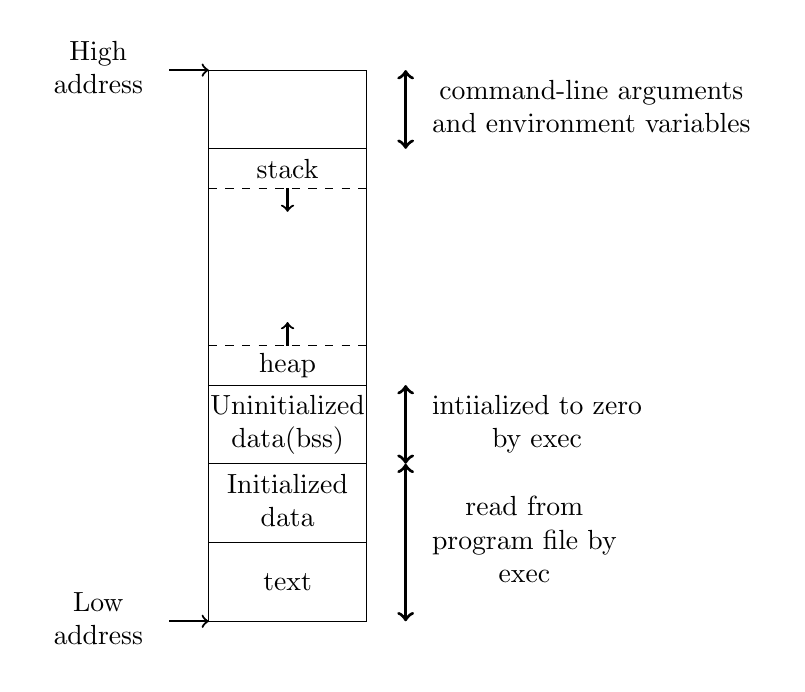
\begin{tikzpicture}
	\draw (0,0) rectangle (2,7);
	\draw [->, thick] (-0.5, 0) -- (0,0);
	\draw [->, thick] (-0.5, 7) -- (0,7);
	\draw (0, 1) -- (2, 1);
	\draw (0, 2) -- (2, 2);
	\draw (0, 3) -- (2, 3);
	\draw [dashed] (0, 3.5) -- (2, 3.5);
	\draw [->, thick] (1,3.5) -- (1,3.8);
	\draw [dashed] (0, 5.5) -- (2, 5.5);
	\draw [->, thick] (1,5.5) -- (1,5.2);
	\draw (0,6) -- (2,6);
	\draw [<->, very thick] (2.5, 6) -- (2.5, 7);
	\draw [<->, very thick] (2.5, 0) -- (2.5, 2);
	\draw [<->, very thick] (2.5, 2) -- (2.5, 3);
	\node at (1, 0.5) {text}; 
	\node at (1, 1.5) {\begin{tabular}{c}Initialized\\data\end{tabular}}; 
	\node at (1, 2.5) {\begin{tabular}{c}Uninitialized\\data(bss)\end{tabular}}; 
	\node at (1, 3.25) {heap};
	\node at (1, 5.75) {stack};
	\node at (-0.5, 0) [anchor = east] {\begin{tabular}{c} Low\\address \end{tabular}};
	\node at (-0.5, 7) [anchor = east] {\begin{tabular}{c} High\\address \end{tabular}};
	\node at (2.5, 6.5) [anchor = west] {\begin{tabular}{c} command-line arguments\\ and environment variables \end{tabular}};
	\node at (2.5, 1) [anchor = west] {\begin{tabular}{c} read from \\ program file by \\ exec \end{tabular}};
	\node at (2.5, 2.5) [anchor = west] {\begin{tabular}{c} intiialized to zero \\ by exec \end{tabular}};
\end{tikzpicture}

In linux the command \texttt{size} can be used to see memory allocation of a compiled C program.\\
Eg: 
 
\begin{mdframed}
	\texttt{\$ size a.out}\\
	\texttt{    text	   data	    bss	    dec	    hex	filename}\\
	\texttt{   1525	    600	      8	   2133	    855	}\\
\end{mdframed}

\textcolor{red}{Where is heap and stack located physically ?}\\
See:\\
\url{https://stackoverflow.com/questions/79923/what-and-where-are-the-stack-and-heap}

\begin{tabularx}{\linewidth}{l|X}
	
\end{tabularx}


\vfill \null
\columnbreak

